\chapter{Fundamentos teóricos} \label{chap:fundamentos-teoricos}

En este Capítulo vamos a dar una introducción a los algoritmos de aprendizaje automático que más adelante usaremos para realizar nuestro análisis con datos reales de laboratorio.

En la Sección \ref{sec:unsupervised} vamos a tratar algunos algoritmos no supervisados, tanto para la reducción de la dimensión de los datos y su visualización, como para la agrupación de los datos en distintas clases, con un número de ellas tanto preestablecido como generado automáticamente a partir de ellos. Posteriormente, en la Sección \ref{sec:supervised} vamos a introducir algoritmos de clasificación supervisada centrándonos en las redes neuronales, tanto secuenciales como convolucionales.

\section{Métodos no supervisados}
\label{sec:unsupervised}

Los algoritmos de aprendizaje automático no supervisados se utilizan cuando no se conoce la salida esperada. Al algoritmo de aprendizaje se le otorgan los datos de entrada y se le pide extraer información de estos datos. Las principales aplicaciones de estos algoritmos, las cuales vamos a aprovechar, son la agrupación de datos y la reducción de dimensionalidad de las variables de los mismos. Esa última es usada principalmente para poder hacer representaciones de datos multidimensionales, los cuales serian complejos de visualizar de otra forma.

La principal pega que pueden tener estos algoritmos es que, si bien no siempre son capaces de identificar conocimiento dados los datos utilizados, cuando lo obtienen, no siempre es el conocimiento que esperábamos obtener. Póngase el ejemplo de un algoritmo que tratase de agrupar rostros de personas iguales. Al no darle a priori ningún tipo de salida de ejemplo, el algoritmo puede acabar clasificando si los rostros están de frente o de lado, no precisamente lo que esperábamos. Es por ello que estos algoritmos cuentan con diversidad de parámetros para ajustarlos a nuestras necesidades, tratando de realizar la agrupación deseada.

En esta sección vamos a estudiar a fondo tres tipos de algoritmos de agrupación: el agrupamiento por k-medias, el agrupamiento aglomerativo, y el agrupamiento por afinidad. Además, estudiaremos también el principal algoritmo de reducción de dimensiones, el análisis de componentes principales, PCA, de sus siglas en inglés. Los principales ejemplos y explicaciones de los algoritmos han sido inspirados por los dados en \cite{machine}.

\begin{mypython}[float={h}, caption={Generar datos artificiales de prueba.}, label={code:artificial-data}]
  from sklearn.datasets import make_blobs

  X, y = make_blobs(n_samples=100, centers=4,
                  n_features=3, random_state=0)
\end{mypython}

Hemos creado un conjunto de datos sintéticos a los cuales poder aplicar todos los algoritmos que vamos a explicar para poder visualizar gráficamente sus resultados. Con la función \texttt{make\_blobs} de Scikit-learn hemos aleatorizado 100 puntos tridimensionales agrupados en cuatro clases fácilmente diferenciables. Scikit-learn es una de las bibliotecas de Python especializada en aprendizaje automático que hemos utilizado. La figura \ref{fig:artificial-data} muestra una representación gráfica del conjunto, y el Código \ref{code:artificial-data} muestra los parámetros que hemos utilizado para crearlo. En la tabla \ref{tab:colab-links} está el enlace para poder ejecutar el código en el \textit{backend} de Google.

% Artificial data
\begin{figure}[h]
  \centering
  \begin{subfigure}{0.45\textwidth}
    \centering
    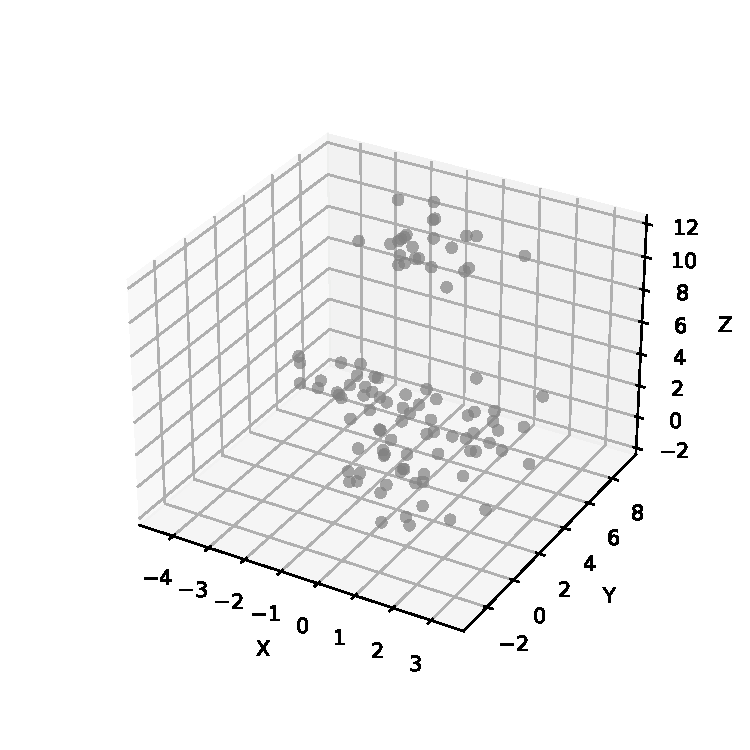
\includegraphics[width=\textwidth]{figures/artificial-data.pdf}
    \caption{}
    \label{fig:artificial-data-grey}
  \end{subfigure}
  \begin{subfigure}{0.45\textwidth}
    \centering
    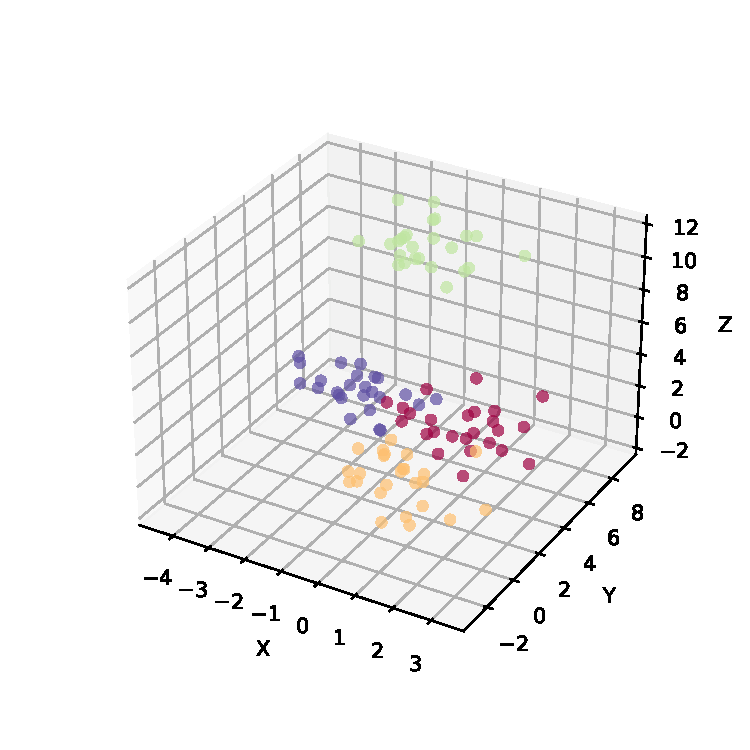
\includegraphics[width=\textwidth]{figures/artificial-data-labeled.pdf}
    \caption{}
    \label{fig:artificial-data-labeled}
  \end{subfigure}
  \caption[Datos artificiales para la prueba de algoritmos.]{Datos artificiales generados para probar algoritmos de agrupamiento. Consisten en 100 puntos tridimensionales agrupados equilibradamente al rededor de 4 centros aleatorios. \ref{fig:artificial-data-grey} En gris los puntos generados sin asignar ninguna etiqueta. Estos serán los datos que recibirán los algoritmos para procesar y agrupar. \ref{fig:artificial-data-labeled} Datos etiquetados según el grupo al que pertenecen. Esto nos ayudará a verificar la eficacia de nuestros algoritmos.}
  \label{fig:artificial-data}
\end{figure}

\subsection{Análisis de componentes principales}

Nuestro conjunto de datos artificiales tiene únicamente 3 dimensiones, lo que hace que sea sencillo poder representarlo gráficamente y que sea fácilmente interpretable. Sin embargo, en la vida real, así como en los datos que en el Capítulo \ref{chap:analisis-y-resultados}, los datos tienden a tener muchas más dimensiones. Esto hace que sea un problema poder representarlos en espacios bidimensionales como este documento, y puede entorpecer también su interpretación o lectura desde otros algoritmos, ya que es probable que haya dimensiones que aporten más ruido que información a la muestra.

Una de las técnicas más utilizadas para tratar este problema es realizar un análisis de componentes principales (PCA) sobre los datos \cite{pca}. Un PCA es una transformación lineal de los datos a un nuevo sistema de coordenadas para facilitar la identificación de las direcciones que contienen más variabilidad. A estas direcciones, que consisten en una combinación lineal de las variables originales, se les denomina \textit{componentes principales}.

El primer paso para realizar un PCA es normalizar los datos para que cada una de las variables originales tenga media 0 y varianza 1. Para ello, denotando $ \textbf{X} = (X_1, ..., X_n) $ a nuestros datos a analizar, donde cada $ X_i $ con $ i \in {1, ..., n} $ es una de las variables de nuestros datos, y $ \mu_{X_i} $ y $ \sigma_{X_i} $ son la media y desviación típica de cada una de las variables, computamos
\begin{equation}
  Z_i = \frac{X_i - \mu_{X_i}}{\sigma_{X_i}},
\end{equation}
para cada $ i $, obteniendo $ \textbf{Z} = (Z_1, ..., Z_n) $ el conjunto de todas nuestras variables normalizadas. Con esto se estandariza la escala de las variables de nuestros datos, evitando que las variables con escalas mayores dominen al resto. En el Código \ref{code:standar} realizamos la normalización de nuestros datos artificiales utilizando la clase \texttt{StandardScaler} de Scikit-learn.

\begin{mypython}[float={h}, caption={Escalar y estandarizar los datos.}, label={code:standar}]
  from sklearn.preprocessing import StandardScaler

  scaler = StandardScaler()
  scaler.fit(X)
  Z = scaler.transform(X)
\end{mypython}

Una vez todos nuestros datos están en la misma escala estamos en disposición de realizar el PCA propiamente dicho. Para ello calculamos la matriz de covarianza $ \Sigma $ de nuestros datos normalizados. $ \Sigma $ es una matriz de dimensión $ n \times n $ con
\begin{equation}
  \Sigma_{ij} = \operatorname{Cov}(Z_{i},Z_{j}) = E[Z_{i}Z_{j}] - E[Z_{i}] E[Z_{j}],
\end{equation}
para $ i, j \in {1, ..., n} $ siendo $ E $ el operador media. Acto seguido, calculamos los $ n $ pares de autovalores y autovectores de la matriz $ \Sigma $ resolviendo la ecuación
\begin{equation}
  \Sigma \textbf{v} = \lambda \textbf{v}.
\end{equation}

Los autovectores $ \textbf{v} $ se denominan componentes principales, y ordenándolos en orden decreciente según el valor de su autovalor $ \lambda $ asociado, obtenemos la lista de componentes principales deseada. Finalmente basta con quedarse con el numero deseado de componentes de la parte superior de la lista para reducir la dimensionalidad de nuestros datos maximizando la covarianza de los mismos. En el Código \ref{code:pca} hemos realizado un PCA de nuestros datos artificiales conservando las 3 componentes principales. Hemos utilizado la clase \texttt{PCA} de Scikit-learn, que encapsula todo el procedimiento que hemos explicado. 

\begin{mypython}[float={h}, caption={Realizar un PCA.}, label={code:pca}]
  from sklearn.decomposition import PCA

  pca = PCA(n_components=3)
  pca.fit(Z)
  Z_pc = pca.transform(X)
\end{mypython}

En la Figura \ref{fig:pca} se muestran gráficamente los puntos artificiales tras el anális de componente principales.

% PCA
\begin{figure}[]
  \centering
  \begin{subfigure}{\textwidth}
    \centering
    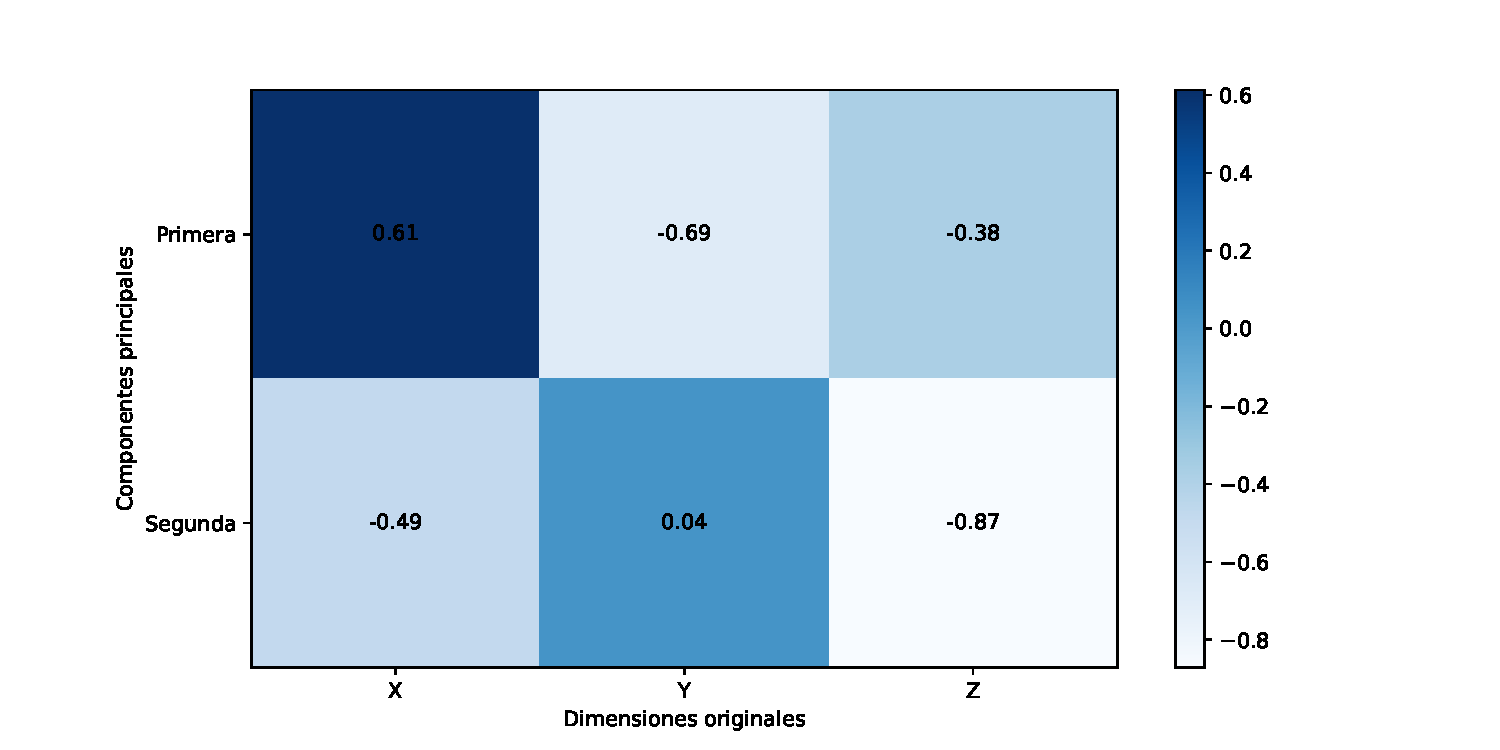
\includegraphics[width=\textwidth]{figures/pca-color-ponderation.pdf}
    \caption{}
    \label{fig:pca-color-ponderation}
  \end{subfigure}
  \begin{subfigure}{0.45\textwidth}
    \centering
    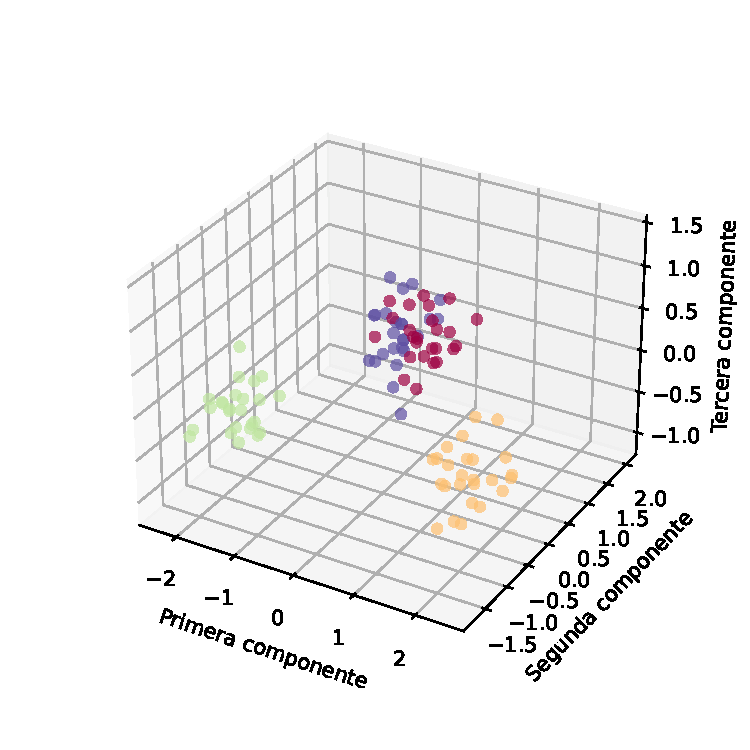
\includegraphics[width=\textwidth]{figures/pca-3d-labeled.pdf}
    \caption{}
    \label{fig:pca-3d-labeled}
  \end{subfigure}
  \begin{subfigure}{0.45\textwidth}
    \centering
    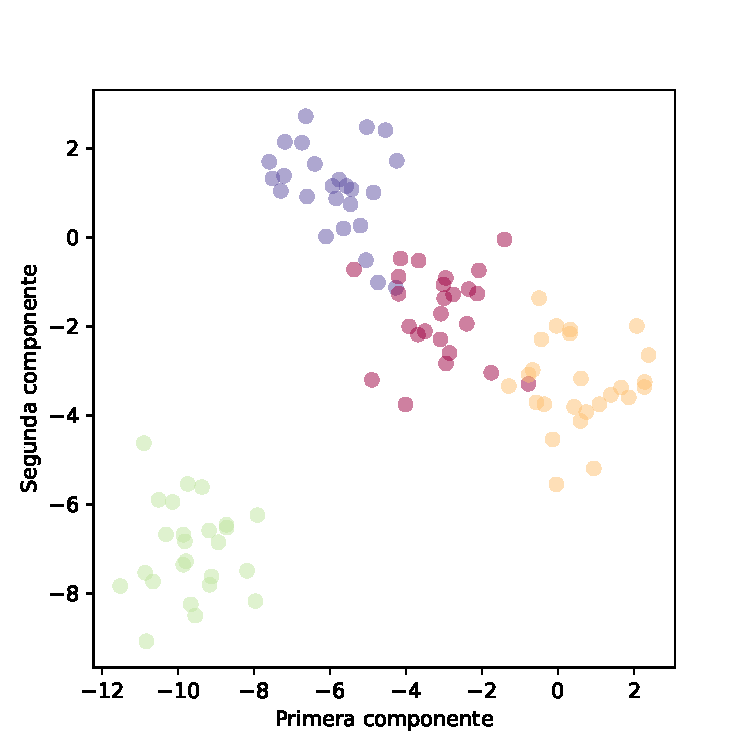
\includegraphics[width=\textwidth]{figures/pca-labeled.pdf}
    \caption{}
    \label{fig:pca-labeled}
  \end{subfigure}
  \caption[Prueba del algoritmo de PCA.]{Prueba del algoritmo de PCA. \ref{fig:pca-color-ponderation} Mapa de calor con las ponderaciones asignadas por el PCA a cada uno de las dimensiones originales. \ref{fig:pca-3d-labeled} Visualización de los datos previamente generados tras escalarlos y aplicarles la PCA. Los colores de los grupos se mantienen, pero los ejes ahora representan las componentes principales, en vez de las dimensiones originales. \ref{fig:pca-labeled} Visualización de las dos primeras componentes principales sobre el plano. Este será el formato en el que visualizaremos más adelante las agrupaciones ejercidas sobre datos reales de dimensionalidad alta.}
  \label{fig:pca}
\end{figure}

\newpage
\subsection{Agrupamiento por k-medias}

El algoritmo de k-medias clasifica los datos separando los datos en $ k $ grupos de manera que la suma de las distancias al cuadrado entre los datos y el centroide del grupo al que pertenecen sea mínima.

El algoritmo comienza inicializando aleatoriamente $ k $ centroides, siendo $ k $ el número de agrupaciones que se le han dicho que realice. Estos centroides serán los centros de las agrupaciones que va a realizar, no tienen por qué pertenecer a los datos, pero sí que están contenidos en su misma dimensión. En cada iteración, el algoritmo asigna a cada punto de los datos el centroide más próximo y luego asigna a cada agrupación un nuevo centroide calculado como la media de los datos que se han asignado a dicha agrupación.

El algoritmo divide un conjunto de $ n $ elementos $ x_j $ en $ k $ agrupaciones disjuntas $ S_i $, cada una descrita por la media $ \mu_k $ de los puntos en la agrupación $ C_k $. Para ello se computan los centroides que 
\begin{equation}
  \underset{C}{\operatorname{arg min}} \sum_{i=1}^k \sum_{x_j \in C_i}  (|| x_j - \mu_i||^2).
\end{equation}

Cuando una iteración no realiza ninguna modificación de las agrupaciones generadas por los centroides de la iteración anterior, el algoritmo finaliza devolviendo las agrupaciones cradas asignando una clase a cada uno de los puntos procesados.

Para computar el algoritmo sobre nuestros datos artificiales hemos utilizado el Código \ref{code:kmeans} usando la clase \texttt{KMeans} de Scikit-learn. Hemos iniciado al algoritmo que separe los datos en dos clases, iniciando los centroides de forma automática. Con esto queremos ver como actúa un algoritmo dividiendo un conjunto de datos generado con 4 clases en mente, cuando se le fuerza a separar únicamente dos grupos.

\begin{mypython}[float={h}, caption={k-medias.}, label={code:kmeans}]
  from sklearn.cluster import KMeans

  kmeans = KMeans(n_clusters=2, n_init="auto")
  kmeans_assigment = kmeans.fit_predict(X)
\end{mypython}

La Figura \ref{fig:kmeans} muestra las dos agrupaciones que se han decidido crear sobre los datos artificiales, simulando lo que más adelante haremos con los datos reales.

% k-means
\begin{figure}[h]
  \centering
  \begin{subfigure}{0.45\textwidth}
    \centering
    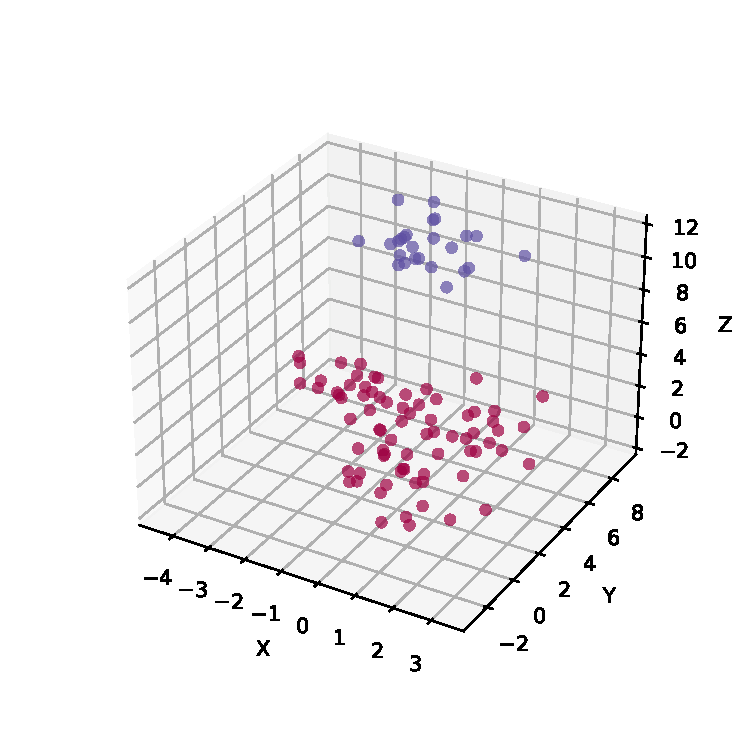
\includegraphics[width=\textwidth]{figures/kmeans-3d.pdf}
    \caption{}
    \label{fig:kmeans-3d}
  \end{subfigure}
  \begin{subfigure}{0.45\textwidth}
    \centering
    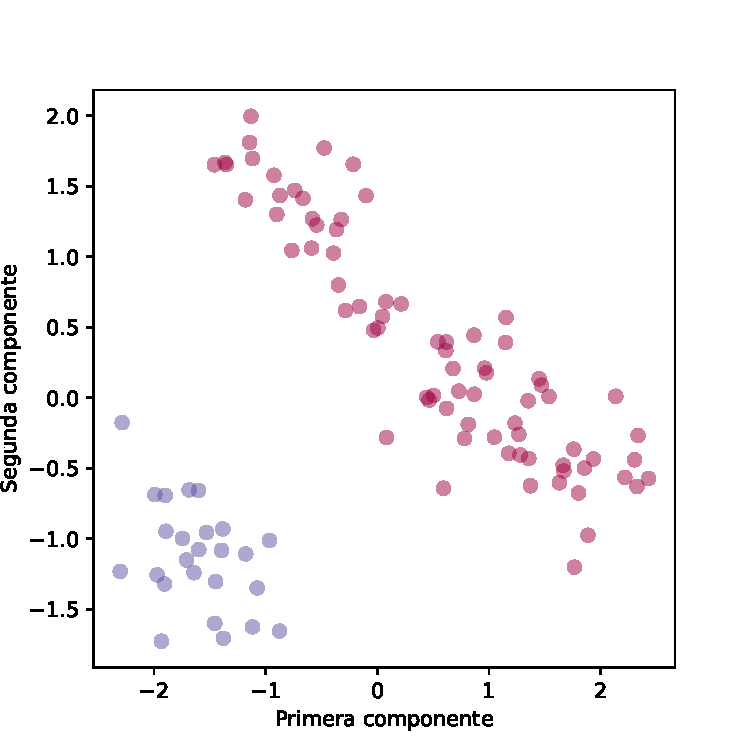
\includegraphics[width=\textwidth]{figures/kmeans-pca.pdf}
    \caption{}
    \label{fig:kmeans-pca}
  \end{subfigure}
  \caption[Prueba del algoritmo de k-medias.]{Prueba del algoritmo de k-medias. \ref{fig:kmeans-3d} Visualización sobre los datos sin modificar de los grupos que ha realizado el algoritmo de k-medias. \ref{fig:kmeans-pca} Visualización de los grupos realizados sobre los datos procesados por el PCA.}
  \label{fig:kmeans}
\end{figure}

\newpage
\subsection{Agrupamiento aglomerativo}

Al igual que el algoritmo de k-medias, el algoritmo de agrupamiento aglomerativo divide los datos dados en el número de grupos indicado. Para ello empieza asignando a cada punto un grupo diferente, para luego ir unificando los grupos en cada iteración según el criterio elegido, hasta alcanzar el número de grupos deseado. Este tipo de algoritmo pertenece a un tipo más amplio de algoritmos denominado agrupación jerárquica, donde además de los agrupamientos aglomerativos están las agrupaciones divisivas. Estas funcionan asignando a todos los puntos el mismo grupo y dividiendo este grupo en cada iteración hasta alcanzar el número deseado.

Los dos tipos de agrupamiento jerárquico funcionan de forma similar, y ambos varían dependiendo de la función de distancia que se utilice, tanto para dividir como para agrupar. Vamos a profundizar en el Método de Ward, que junta los grupos que al juntarse minimicen la varianza mínima dentro del nuevo grupo. Así, la varianza de un grupo $ C $ de puntos $ \{x_1, ..., x_n\} $ se define como
\begin{equation}
  V(C) = \sum\limits_{i=1}^n || x_i - \mu_C ||^2,
\end{equation}
siendo $ \mu_C $ la media de los puntos del grupo $ C $.

Por tanto, en cada iteración el algoritmo calcula el incremento de varianza que supondría juntar cada par de grupos $ A $ y $ B $ calculando
\begin{equation}
  \delta(A, B) = \frac{|A||B|}{|A|+|B|}||\mu_A - \mu_B||^2,
\end{equation}
donde $ |\cdot| $ denota el cardinal de los grupos y $ || \cdot || $ la operación módulo.

Tras ello, unifica los dos grupos que supongan un menor incremento en la varianza y repite el proceso hasta obtener el número deseado de grupos.

\begin{mypython}[float={h}, caption={Agrupamiento aglomerativo.}, label={code:agglomerative}]
  from sklearn.cluster import AgglomerativeClustering

  agg = AgglomerativeClustering()
  agg_assigment = agg.fit_predict(X)
\end{mypython}

En el Código \ref{code:agglomerative} hemos realizado un agrupamiento aglomerado sobre nuestros puntos artificiales utilizando la clase \texttt{AgglomerativeClustering} de Scikit-learn, que por defecto, si no se le indica lo contrario, utiliza el Método de Ward en la ejecución del algoritmo. En la Figura \ref{fig:agglomerative} se muestran los resultados sobre nuestros datos de forma gráfica.

% Agglomerative
\begin{figure}[h]
  \centering
  \begin{subfigure}{0.45\textwidth}
    \centering
    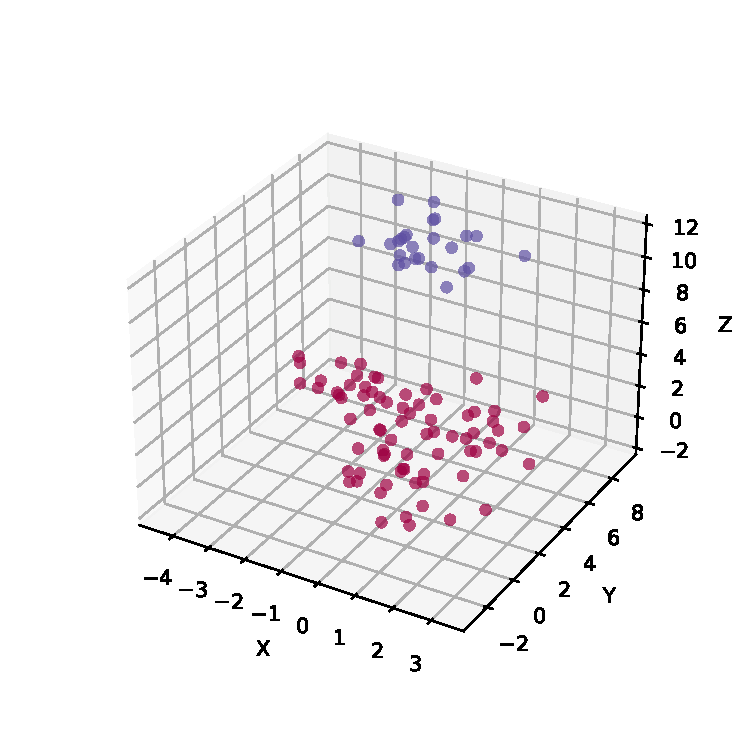
\includegraphics[width=\textwidth]{figures/agglomerative-3d.pdf}
    \caption{}
    \label{fig:agg-3d}
  \end{subfigure}
  \begin{subfigure}{0.45\textwidth}
    \centering
    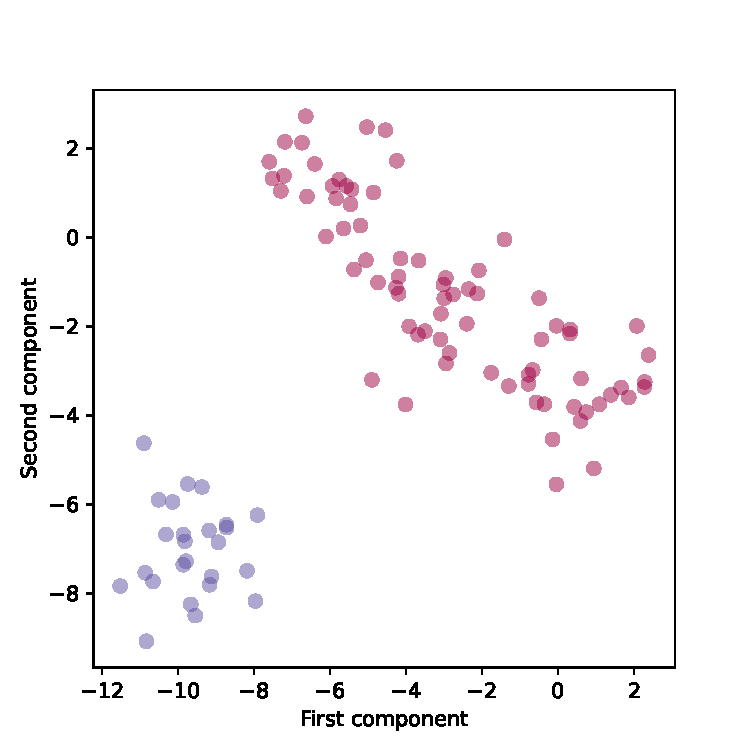
\includegraphics[width=\textwidth]{figures/aglomerative-pca.pdf}
    \caption{}
    \label{fig:agg-pca}
  \end{subfigure}
  \caption[Prueba del algoritmo de agrupamiento aglomerado.]{Prueba del algoritmo de agrupamiento aglomerado. \ref{fig:agg-3d} Visualización sobre los datos sin modificar de los grupos que ha realizado el algoritmo. \ref{fig:agg-pca} Visualización de los grupos realizados sobre los datos procesados por el PCA.}
  \label{fig:agglomerative}
\end{figure}

\newpage
\subsection{Agrupamiento por propagación de afinidad}

El algoritmo de propagación de afinidad \cite{affinity} crea agrupaciones mandando mensajes entre pares de puntos hasta que converge. La principal cualidad de este algoritmo es que, a diferencia con la mayoría de algoritmos de agrupamiento, no necesita saber el número de agrupaciones a realizar de antemano, sino que las genera dinámicamente. Consigue esto ya que, a diferencia de algoritmos como el agrupamiento por k-medias, que inicializa tantos centroides como grupos se quieran obtener, el algoritmo de propagación de afinidad empieza considerando como posibles centroides a todos los puntos de la muestra.

Para ello, el algoritmo se inicializa con una matriz de afinidad $ S $, formada por los valores de afinidad $ s(i, k) $ que indican lo apropiado que sería escoger el dato $ k $ como ejemplar del dato $ i $. Esta matriz puede inicializarse de multitud de formas, pero por defecto se utiliza el negativo de la distancia Euclídea al cuadrado. Con ella, para los puntos $ x_i $, $ x_k $, se tendría
\begin{equation}
  s(i, k) = -||x_i - x_k||^2.
\end{equation}

El algoritmo se ejecuta actualizando dos matrices por medio de \textit{mensajes} hasta que se estabiliza o llega a un número máximo de iteraciones. La \textit{matriz de responsabilidad} $ R $ con valores $ r(i, k) $ cuantifica la evidencia acumulada de como de apropiado es escoger $ x_k $ para ser el ejemplar de $ x_i $. Y la \textit{matriz de disponibilidad} $ A $ con valores $ a(i, k) $ que refleja la evidencia acumulada de como de apropiado sería que un punto $ x_i $ escogiera a un punto $ x_k $ como ejemplar.

Ambas matrices se inicializan a cero y en cada iteración se actualiza primero la matriz de responsabilidad
\begin{equation}
  r(i, k) \leftarrow s(i, k) - \underset{k' \neq k}{\operatorname{max}}\{a(i, k') + s(i, k')\},
\end{equation}
después la matriz de disponibilidad para $ i \neq k $
\begin{equation}
  a(i, k) \leftarrow \operatorname{min}\left\{0, r(k, k) + \sum_{i' \notin \{i, k\}} \operatorname{max}\{0, r(i', k)\}\right\},
\end{equation}
y para el resto de casos
\begin{equation}
  a(k, k) \leftarrow \sum_{i' \neq k} \operatorname{max}\{0, r(i', k)\}.
\end{equation}

Tras alcanzar el criterio de parada se eligen los puntos $ x_k $ para los cuales
\begin{equation}
  a(k, k) + r(k, k) > 0,
\end{equation}
como puntos ejemplares determinando el número de grupos obtenidos y asignando al resto de puntos el grupo de cuyo ejemplar sean más similares.

\begin{mypython}[float={h}, caption={Propagación de afinidad.}, label={code:aff}]
  from sklearn.cluster import AffinityPropagation

  aff = AffinityPropagation()
  aff_assigment = aff.fit_predict(X)
\end{mypython}

En el Código \ref{code:aff} hemos utilizado la clase \texttt{AffinityPropagation} de Scikit-learn para realizar un agrupamiento por propagación de afinidad sobre nuestros datos artificiales. En la Figura \ref{fig:aff} vemos los resultados del agrupamiento, observando como sin haber indicado el número de grupos deseado, el algoritmo consigue diferenciar los cuatro grupos planteados por el generador de datos.

% Affinity
\begin{figure}[h]
  \centering
  \begin{subfigure}{0.45\textwidth}
    \centering
    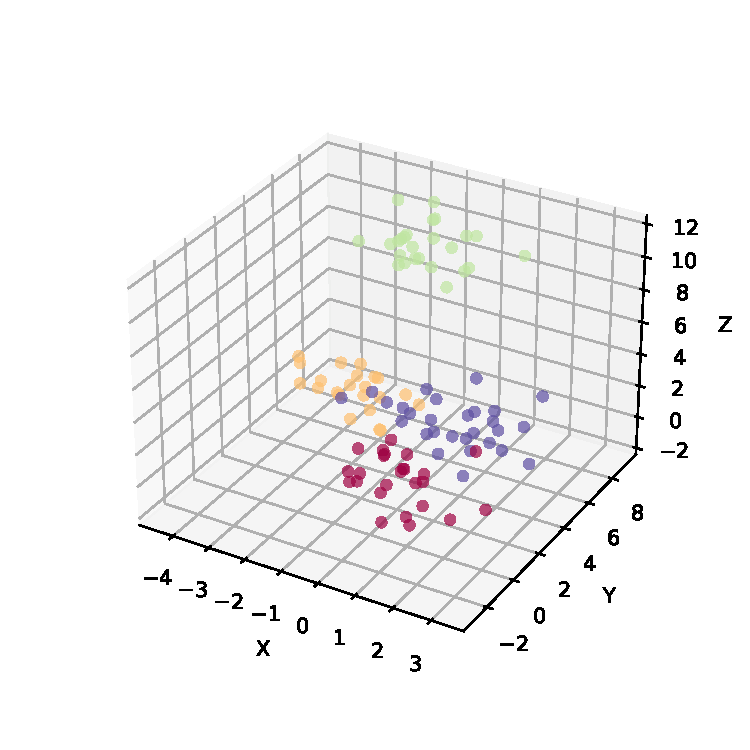
\includegraphics[width=\textwidth]{figures/affinity-3d.pdf}
    \caption{}
    \label{fig:aff-3d}
  \end{subfigure}
  \begin{subfigure}{0.45\textwidth}
    \centering
    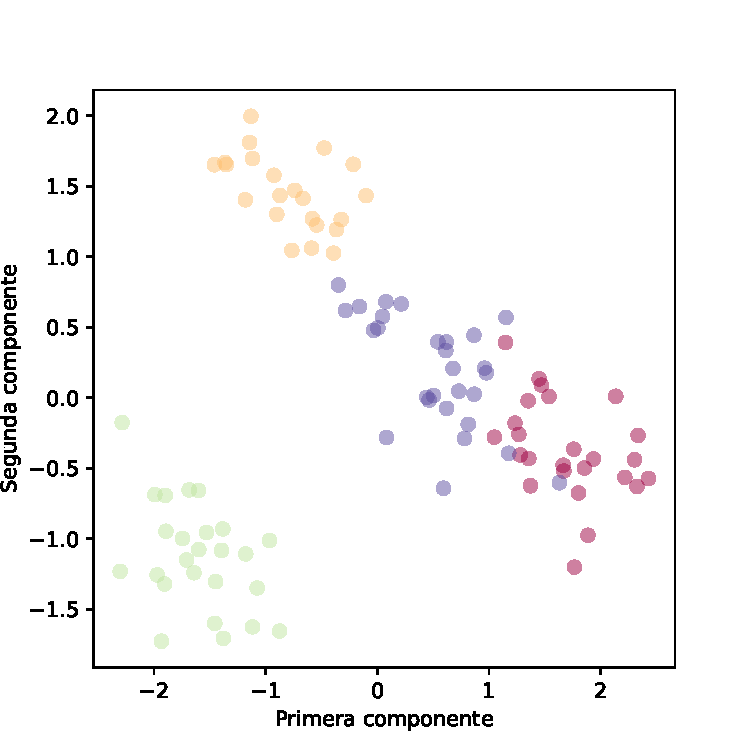
\includegraphics[width=\textwidth]{figures/affinity-pca.pdf}
    \caption{}
    \label{fig:aff-pca}
  \end{subfigure}
  \caption[Prueba del algoritmo de propagación de afinidad.]{Prueba del algoritmo de propagación de afinidad. \ref{fig:aff-3d} Visualización sobre los datos sin modificar de los grupos que ha realizado el algoritmo. \ref{fig:aff-pca} Visualización de los grupos realizados sobre los datos procesados por el PCA.}
  \label{fig:aff}
\end{figure}

\newpage
\section{Métodos supervisados}
\label{sec:supervised}

Al contrario que los métodos de aprendizaje automático no supervisados, donde no sabemos de antemano la salida deseada, los métodos de aprendizaje automático supervisados permiten calibrar los modelos utilizando los datos de salida que queremos mediante el uso de datos de entrenamiento de los cuales conocemos su salida esperada. Para métodos de agrupamiento y separación de clases como los que nos interesan en este trabajo, basta con contar con un conjunto de datos previamente etiquetado con su clase real como datos de entrenamiento, permitiendo a los modelos aprender sobre la clasificación dada y posteriormente replicarla para datos nuevos.

En el laboratorio contamos con datos de sesiones etiquetadas con el estado del tratamiento de los animales, por lo que pueden servir para entrenar un método supervisado. En esta sección, contamos con los datos artificiales que hemos generado, en los cuales cada punto tiene asignado uno de cuatro grupos diferentes.

Existen multitud de métodos no supervisados, sin embargo vamos a centrarnos únicamente en el que más está siendo utilizado a día de hoy, dando buenos resultados en múltiples disciplinas para todo tipo de problemas: las redes neuronales. En esta sección vamos a introducir primero el ejemplo fundamental de redes neuronales, las redes neuronales secuenciales, para luego hablar de las redes neuronales convolucionales, que serán las que finalmente apliquemos a nuestros datos reales. Los ejemplos y explicaciones se basan en los de \cite{understanding} y \cite{pytorch}.

\subsection{Red neuronal secuencial}

Antes de profundizar en el concepto de red, es necesario definir las piezas por las cuales están formadas, las \textit{neuronas artificiales}. Una neurona es una función que recibe un vector de entradas $ \mathbf{x} = (x_1, ..., x_n) $ y asigna un peso a cada una de ellas, representados mediante un vector de pesos $ \mathbf{w} = (w_1, ..., w_n) $, mediante una combinación lineal, sumando además un sesgo $ b $,
\begin{equation}
  z = \sum_{i=1}^n w_i x_i + b = \mathbf{w} \cdot \mathbf{x} + b.
\end{equation}

El resultado de esta combinación lineal pasa después por una función de activación $ \varphi(z) $ que lo filtra antes de obtener la salida final de la neurona
\begin{equation}
  y = \varphi(\mathbf{w} \cdot \mathbf{x} + b).
\end{equation}

La función de activación $ \varphi $ varía en función del problema que se quiera tratar y del diseño de la red. Algunos de los ejemplos más comunes son la tangente hiperbólica (tanh)
\begin{equation}
  \varphi(z) = \operatorname{tanh}(z) = \frac{e^z - e^{-z}}{e^z + e^{-z}},
\end{equation}
la cual vamos a usar en las pruebas de esta sección, o el rectificador linear unitario (ReLu),
\begin{equation}
  \varphi(z) = \operatorname{max}(0, z),
\end{equation}
el cual es ampliamente utilizado por sus buenos resultados en problemas generales, y hemos utilizado en la Sección \ref{sec:analisis} con nuestros datos reales.

Una vez definido el concepto de neurona podemos definir una red \textit{neuronal secuencial completa} como un conjunto de neuronas divididas en diferentes capas. En la primera capa, la \textit{capa de entrada}, cada neurona recibe como entrada todos los datos a procesar y manda su salida a la entrada de cada una de las neuronas de la siguiente capa. En las capas intermedias, \textit{capas ocultas}, las neuronas reciben un vector de entrada formado por las salidas de la capa anterior, y vuelven a pasar su salida a las capas posteriores. Finalmente, la última capa, la \textit{capa de salida}, recibe su entrada de la capa anterior y devuelve la salida final de la red. En función del número de neuronas de esta capa, la red podrá devolver más o menos información. En la Figura \ref{fig:diagram-sec} se muestra un ejemplo de una posible red neuronal secuencial.

\begin{figure}[h]
  \centering
  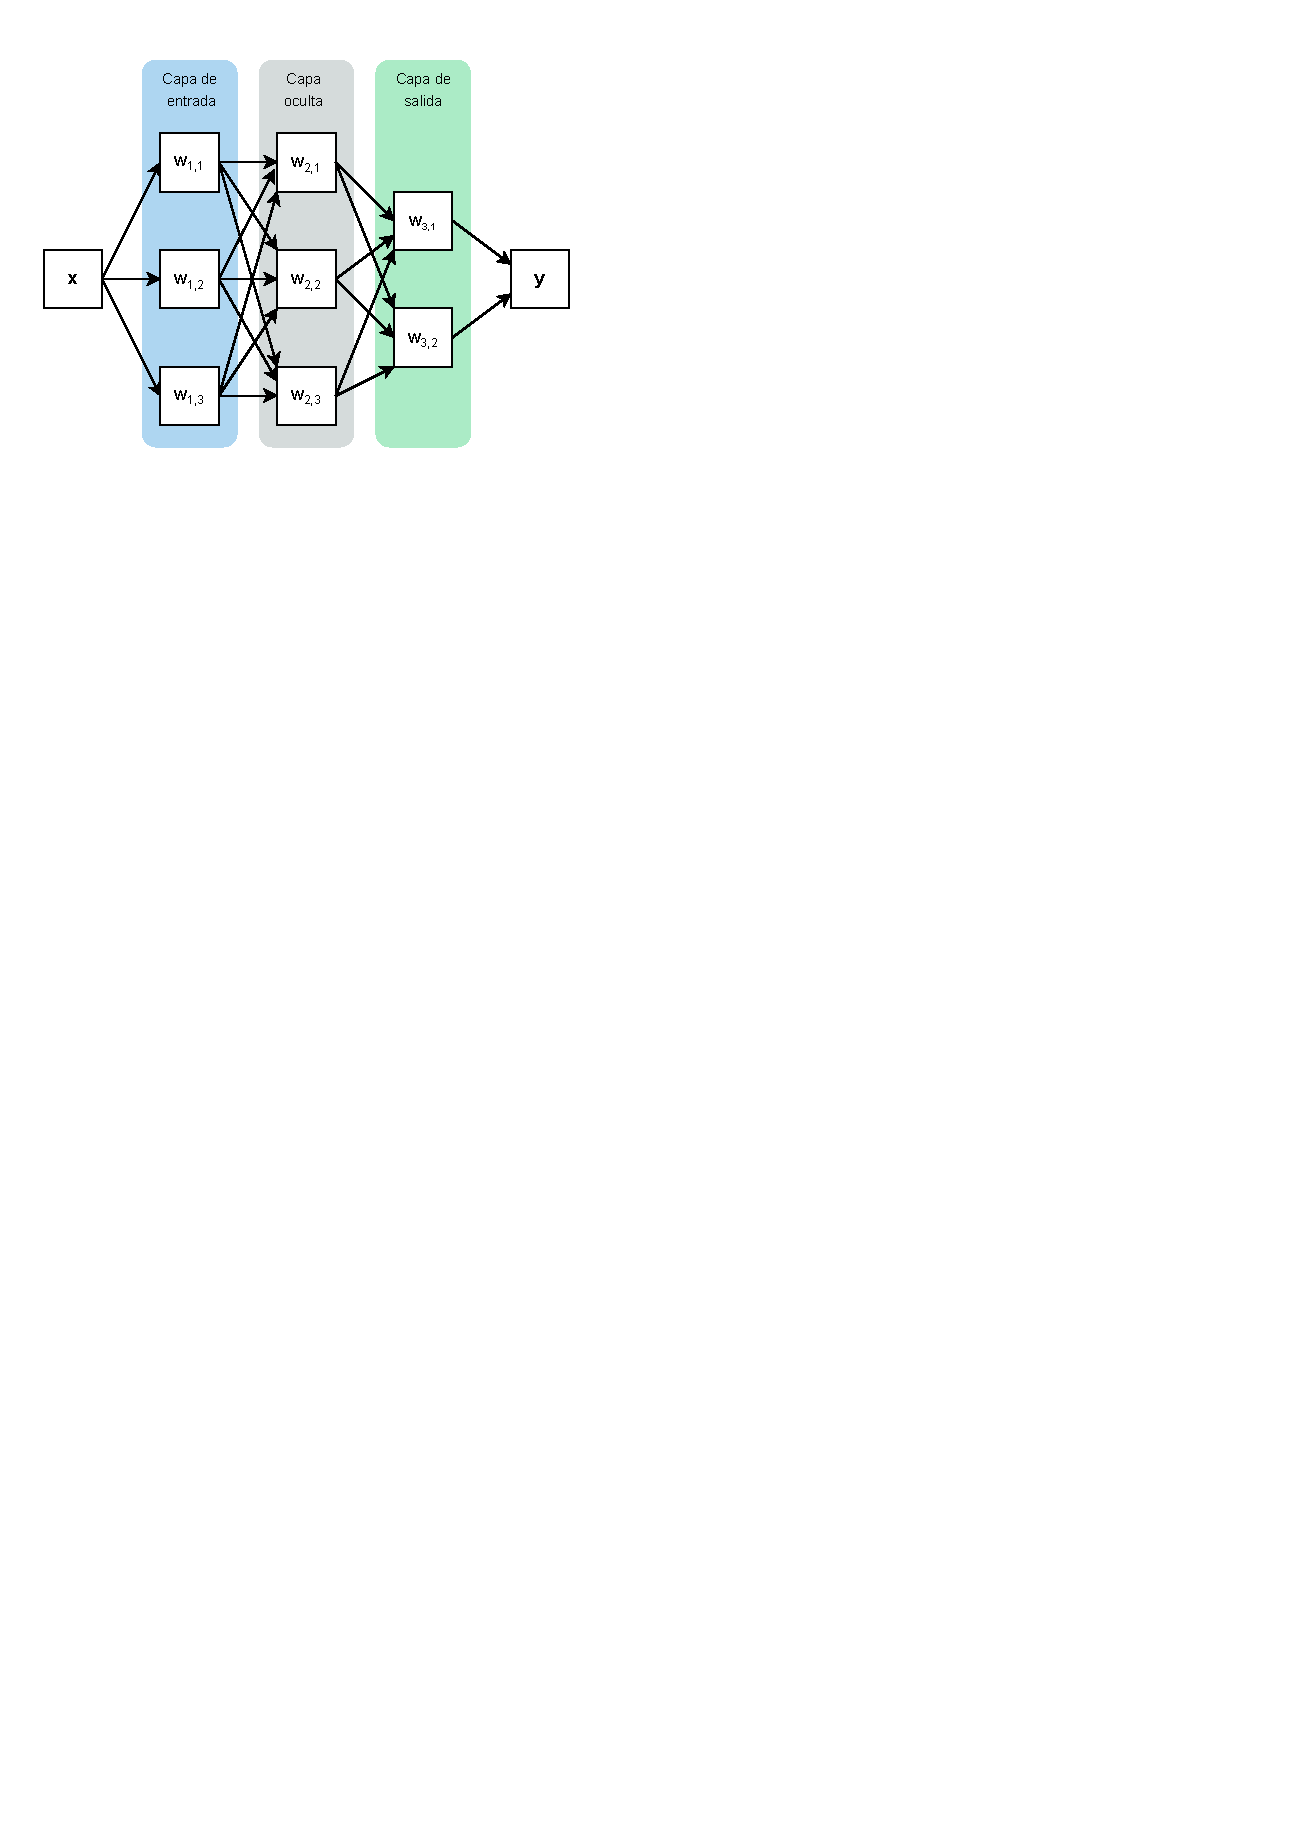
\includegraphics{figures/diagram-secuential.pdf}
  \caption{Diagrama simplificado de una red secuencial. En esta red, la capa de entrada (azul) tiene tres neuronas que reciben los datos de $ \mathbf{x} $ y tras aplicar los pesos, el sesgo y la función de activación, pasan a una capa oculta (gris). Esta capa recibe todas las salidas de la capa anterior y tras repetir el procedimiento anterior, pasa su salida a la capa de salida (verde). En este caso, tiene solo dos neuronas, definiendo el tamaño de los datos de la salida $ \mathbf{y} $ de la red.}
  \label{fig:diagram-sec}
\end{figure}

Para clasificar datos mediante una red neuronal es necesario contar con un conjunto de datos etiquetado dividido en un conjunto de entrenamiento y otro conjunto de validación, para poder así \textit{entrenar} nuestra red y validar la calidad de su aprendizaje. Así, se empieza inicializando los valores de los pesos de la red a valores predeterminados, y luego se empiezan a propagar hacia delante los datos de entrenamiento calculando el error $ L $ cometido al clasificarlos comparando la salida de la red con el valor de su clasificación real
\begin{equation}
  L = \frac{1}{m} \sum_{i=1}^{m}(y_i - \hat{y}_i)^2,
\end{equation}
donde $ m $ es el número de neuronas de la capa de salida y $ \hat{y}_i $ es la salida esperada en cada una de esas neuronas para cada vector de entrada propagado hacia delante.

El siguiente paso es propagar el error hacia detrás calculando el error relativo cometido por cada una de las neuronas, para poder así modificar sus pesos y sesgos. Se calcula el gradiente de $ L $ calculando la derivada parcial de $ L $ respecto a cada uno de los pesos $ \mathbf{w} $ y el sesgo $ b $ y se actualizan los parámetros introduciendo un \textit{ratio de aprendizaje} $ \alpha $. Denotando $ \phi \in \{\text{pesos y sesgos}\} $ a cualquiera de los parámetros de las distintas neuronas, tenemos que en cada iteración cada parámetro $ \phi $ se actualiza
\begin{equation}
  \phi \leftarrow \phi - \alpha \cdot \frac{\partial L}{\partial \phi}.
\end{equation}
Este proceso se repite hasta obtener un error aceptable y dar por concluido el entrenamiento de la red. Después, se comprueba su eficacia y su capacidad de aprendizaje y adaptación a casos nuevos verificando su comportamiento con los datos reservados para la validación.

Para implementar una red neuronal de estas características utilizando PyTorch, en el Código \ref{code:dataset} hemos creado una clase heredada del objeto \texttt{Dataset} de PyTorch, en la cual almacenamos nuestros datos y sus respectivas clases a la vez, accediendo a los datos en formato de \texttt{tensor}, el tipo de dato de PyTorch optimizado para operaciones en GPU.

\begin{mypython}[float={h}, caption={\texttt{Dataset} de los datos artificiales.}, label={code:dataset}]
from torchvision import torch
from torch.utils.data import Dataset

class RawDataset(Dataset):
  def __init__(self, arr, labels):
      self.data = arr
      self.labels = labels

  def __len__(self):
      return len(self.data)

  def __getitem__(self, idx):
      data = self.data[idx]
      label = self.labels[idx]
      return torch.tensor(data, dtype=torch.float), label

dataset = RawDataset(X, y)
\end{mypython}

Para inicializar nuestros datos de entrenamiento y validación, en el Código \ref{code:train-val-data} utilizamos la función \texttt{random\_split}, que se encarga de distribuir nuestros puntos de forma aleatoria en los distintos subconjuntos. Además, fijamos el tamaño de los lotes que vamos a pasar a la red durante el entrenamiento, antes de actualizar los parámetros minimizando la función de pérdida, e inicializamos dos \texttt{DataLoader} que se encargaran de seleccionar aleatoriamente y en el tamaño de lote seleccionado, datos para pasar a la red tanto en el entrenamiento como en la validación.

\begin{mypython}[float={h}, caption={Inicialización de los conjuntos de entrenamiento y validación.}, label={code:train-val-data}]
from torch.utils.data import DataLoader, random_split

train_size = int(0.8 * len(dataset))
test_size = len(dataset) - train_size 

train_dataset, test_dataset = \
  random_split(dataset, [train_size, test_size])

batch_size = 3
train_loader = DataLoader(train_dataset,
                          batch_size=batch_size,
                          shuffle=True)
test_loader = DataLoader(test_dataset,
                         batch_size=batch_size, 
                         shuffle=False)
\end{mypython}

Finalmente, en el Código \ref{code:model} inicializamos nuestra red con dos capas lineales y una función de activación \texttt{Tanh} entre medias. La primera capa tiene 3 entradas, una por cada variable de los puntos artificiales y un número arbitrario de 128 salidas. Tras pasar por la función de activación, la segunda capa recibe esas 128 salidas de la capa anterior como sus entradas y saca 4 salidas, una por cada grupo que queremos distinguir.

Posteriormente se escogen una función de pérdida y un optimizador de entre los proporcionados por PyTorch, y se fijan la tasa de aprendizaje y el número de iteraciones que se quieren realizar.

Una vez todos los componentes están listos, se itera en el bucle principal tantas veces como se desee ejecutando los pasos de entrenamiento explicados previamente. En la Figura \ref{fig:net-artificial} se observan los resultados de la validación, observando que esta red básica es suficiente para clasificar todos los dato de validación correctamente.

\begin{mypython}[float={h}, caption={Modelo de la red y enrenamiento con los datos artificiales.}, label={code:model}]
import torch.nn as nn

model = nn.Sequential(
  nn.Linear(3, 128),
  nn.Tanh(),
  nn.Linear(128, 4))
loss_fn = nn.CrossEntropyLoss()
learn_rate = 1e-2
optimizer = torch.optim.SGD(model.parameters(), lr=learn_rate)
n_epochs = 100

for epoch in range(n_epochs):
  for sessions, labels in train_loader:
    batch_size = sessions.shape[0]
    outputs = model(sessions.view(batch_size, -1))

    loss = loss_fn(outputs, labels)
    optimizer.zero_grad()
    loss.backward()
    optimizer.step()
\end{mypython}

% Net
\begin{figure}[p]
  \centering
  \begin{subfigure}{0.45\textwidth}
    \centering
    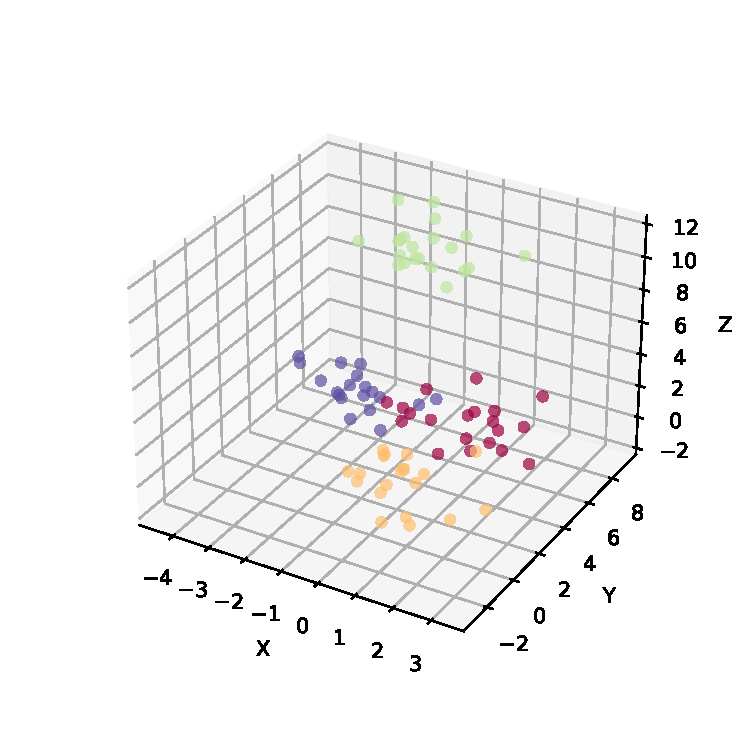
\includegraphics[width=\textwidth]{figures/train-asig-artificial.pdf}
    \caption{}
    \label{fig:train-artificial}
  \end{subfigure}
  \begin{subfigure}{0.45\textwidth}
    \centering
    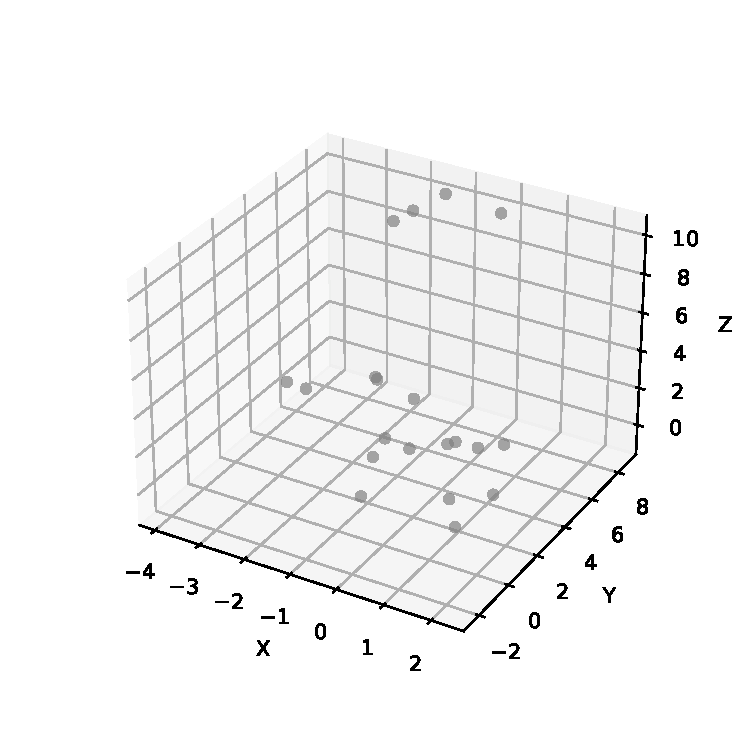
\includegraphics[width=\textwidth]{figures/test-artificial.pdf}
    \caption{}
    \label{fig:test-artificial}
  \end{subfigure}
  \begin{subfigure}{0.45\textwidth}
    \centering
    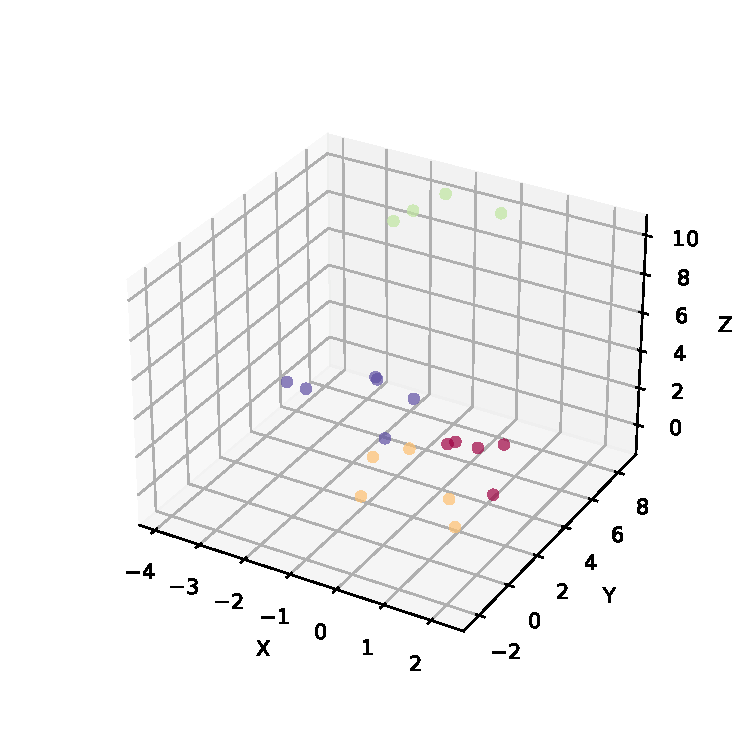
\includegraphics[width=\textwidth]{figures/test-asig-artificial.pdf}
    \caption{}
    \label{fig:net-class-artificial}
  \end{subfigure}
  \caption[Prueba de red neuronal secuencial.]{Prueba de clasificación mediante una red neuronal secuencial. \ref{fig:train-artificial}: Subconjunto de entrenamiento de los datos artificiales. Generado seleccionando 80 puntos de forma aleatoria manteniendo la información del grupo al que pertenecen para realizar el entrenamiento de nuestra red secuencial. \ref{fig:test-artificial}: Subconjunto de validación de los datos artificiales. Formado por los 20 puntos restantes que no se han seleccionado para el subconjunto de entrenamiento. Se guarda la información de sus grupos originales, pero no se le pasa a la red, para así obtener una clasificación automática y poder posteriormente verificar los resultados. \ref{fig:net-class-artificial}: Clasificación de los datos de validación generada por la red. Acierta el grupo real de los 20 puntos con los que se ha verificado su comportamiento.}
  \label{fig:net-artificial}
\end{figure}

\newpage
\subsection{Red neuronal convolucional}
Para resolver problemas simples como la clasificación de los puntos artificiales con los que hemos estado trabajando, las redes neuronales secuenciales lineales como la que hemos visto funcionan perfectamente, sin embargo, a la hora de analizar datos reales no siempre consiguen los resultados que nos gustaría. Para arreglar esto se puede valorar aumentar el número de capas de la red, aumentar el tamaño de las capas, probar diferentes funciones de activación, o aumentar el número de datos de entrenamiento. Otra posible opción es probar con redes que funcionen algo diferente como, por ejemplo, las redes neuronales convolucionales.

Las redes secuenciales relacionan cada punto del vector de entrada con todos los demás \texttt{asumiendo} que pueden existir relaciones entre cualquier par de puntos. Las redes convolucionales, en cambio, incorporan capas encargadas de aplicar una serie de filtros sobre los datos para asociar y dar relevancia a puntos próximos entre sí. Las redes convolucionales son ampliamente utilizadas para el análisis de imágenes, ya que es frecuente que las estructuras y características que podamos querer buscar en una imagen, estén formadas por píxeles próximos entre sí. En nuestro caso, vamos a analizar datos en series temporales, por lo que de la misma forma, es probable que las estructuras que queremos encontrar estén próximas temporalmente.

\begin{figure}[h]
  \centering
  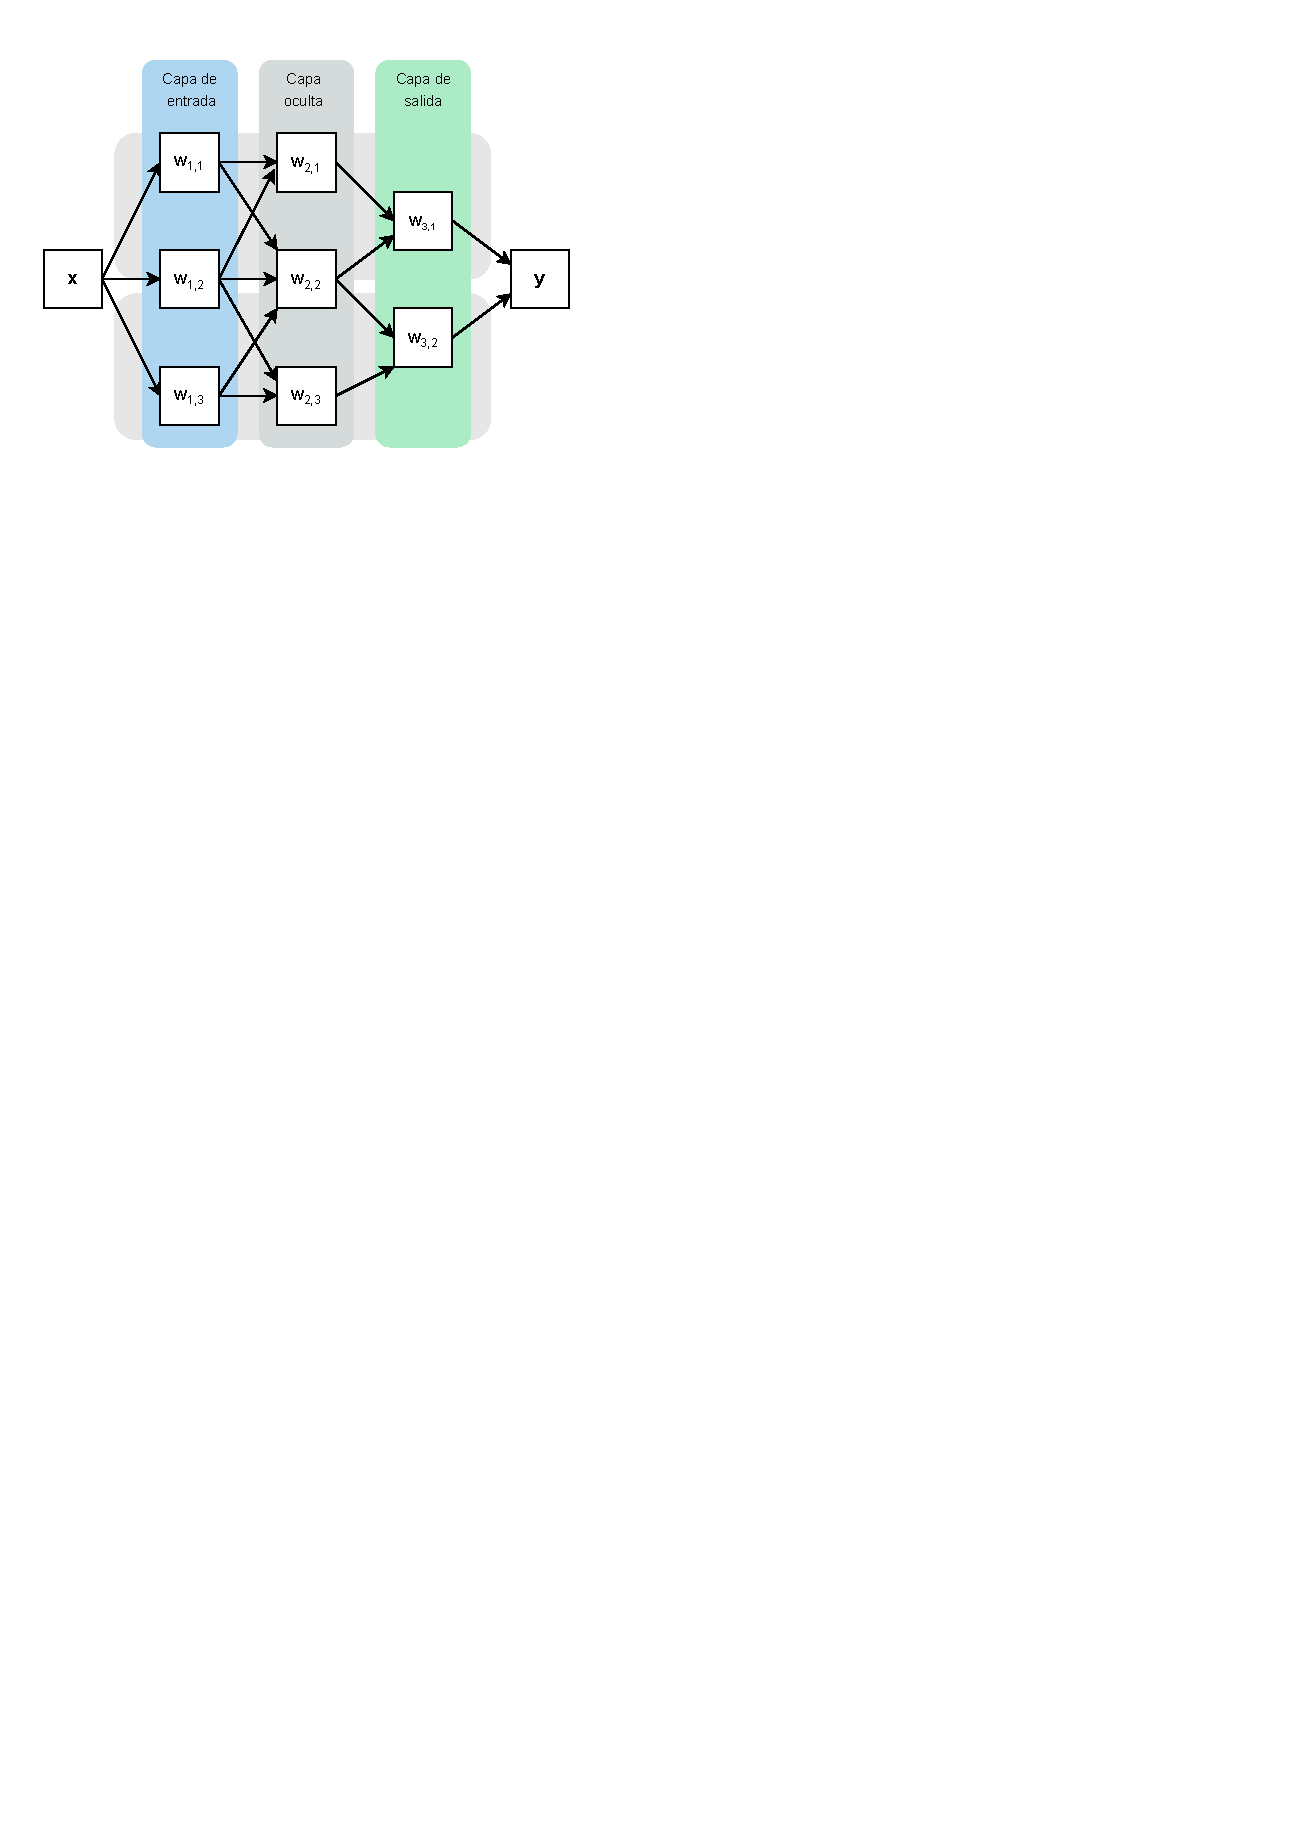
\includegraphics{figures/diagram-convolutional.pdf}
  \caption{Diagrama simplificado de una red convolucional. Partiendo de la red secuencial de la Figura \ref{fig:diagram-sec} se han modificado las capas por capas convolucionales. De esta forma, cada una de las neuronas solo pasa información a neuronas cercanas, relacionando los datos próximos de $ \mathbf{x} $.}
  \label{fig:diagram-conv}
\end{figure}

La Figura \ref{fig:diagram-conv} muestra una red convolucional simplificada construida a partir de la estructura de la red secuencial vista previamente. No vamos a centrarnos a fondo en los detalles matemáticos de estas redes, pero en la Sección \ref{sec:analisis} vamos a implementar una red convolucional a medida para nuestros datos de laboratorio utilizando PyTorch.